\section{Introduction into Parallel Genetic Algorithms}
\label{cha:teoria}
\subsection{Basic notation used in $\mathcal{GA}$}
\label{cha:BasicNotation}
$\mathcal{GA}$ (Genetic Algorithm) is a search algorithm inspired by genetics and
natural selection. At first it is worth introducing few basic notions connected
with this topic \cite{bib10}:
\begin{itemize}
	\item Reproduction is the process by which the genetic material in two or
		more parent individual is combined to obtain one or more offspring.
	\item Mutation is applied to one individual in order to produce a new
		version of it where some of the original genetic material has been
		randomly changed
	\item Fitness evaluation is the step in which the quality of individual is
		assessed.
	\item Selection is an operation used to decide which individuals use for
		reproduction
	\item Crossover is the basic genetic operator; it randomly chooses at least two
		individuals and with a given probability exchanges their genomes to
		create new individuals. 
	\item Offspring population- population which was created by the work of
		genetic operators.
	\item Gene- rudimentary unit building the chromosome. It encodes information
		about individual
	\item Chromosome- unit which builds the genotype of the individual, contains
		information used to identify phenotype and it can encode additional
		parameters which are not used in fitness evaluation. 
	\item Genotype- information about the individual which directly defines its
		positions in the solution space 
	\item Environment- entire solution space defined according to the problem to solve. 
\end{itemize}

\subsection{Multiprocessor system taxonomy}
\label{cha:MultiprocessorTaxonomy}
There are many ways to classify parallel computers \cite{bib20}. One of the most widely used
classification, known since 1966, is called Flynn's Taxonomy \cite{bib15}. It distinguishes
multi-processor architecture by taking into account two independent domains.
They are instruction and data domains with two possible states: Single or Multiple. This topic is
very important in case of parallel genetic realisation, but this area fall
outside the scope of this thesis. Summary presented
below is only placed here to enlighten the problem.
We can distinguish four basic combinations:
\begin{enumerate}
	\item Single Instruction, Single Data $\mathcal{SISD}$
		\begin{enumerate}
			\item A serial (non-parallel) computer 
			\item Single instruction: only one instruction stream is being acted on the CPU during any one clock cycle 
			\item Single data: only one data stream is being used as input during any one clock cycle 
			\item Deterministic execution 
			\item This is the oldest and even today, the most common type of computer 
		\end{enumerate}
	\item Single Instruction, Multiple Data $\mathcal{SIMD}$
		\begin{enumerate}
			\item A type of parallel computer 
			\item Single instruction: All processing units execute the same instruction at any given 
				clock cycle 
			\item Multiple data: Each processing unit can operate on a different data element 
			\item Best suited for specialized problems characterized by a high degree of regularity, 
				  such as graphics/image processing. 
			\item Synchronous (lockstep) and deterministic execution 
			\item Two variants: Processor Arrays and Vector Pipelines 
		\end{enumerate}
	\item Multiple Instruction, Single Data $\mathcal{MISD}$
		\begin{enumerate}
			\item A single data stream is fed into multiple processing units. 
			\item Each processing unit operates on the data independently via independent instruction streams.
		\end{enumerate}
	\item Multiple Instruction, Multiple Data $\mathcal{MIMD}$
		\begin{enumerate}
			\item Currently, the most common type of parallel computer. Most modern computers fall into this category. 
			\item Multiple Instruction: every processor may be executing a different instruction stream 
			\item Multiple Data: every processor may be working with a different data stream 
			\item Execution can be synchronous or asynchronous, deterministic or non-deterministic 
		\end{enumerate}
\end{enumerate}

\subsection{Overview of $\mathcal{PGA}$ taxonomy }
\label{cha:PgaTaxonomy}

\subsubsection{Sequential versus parallel $\mathcal{GA}$ implementations}
\label{cha:GaDifference}
When using the term parallel genetic algorithm it is important to distinguish between parallel models,
their (parallel or sequential) implementation, and the computer hardware
parallelization \cite{bib20}. A traditional sequential $\mathcal{GA}$ model has a single population and no restrictions
upon which strings recombine with which. In a parallel $\mathcal{GA}$ model there are either multiple
populations (an island model) or a~partitioning of a single population (often called a fine-grained model). 
Both parallel and sequential $\mathcal{GA}$ models can have parallel or sequential implementations.
A~sequential implementation of the global model is the traditional approach discussed 
in the literature. One process, running on a uniprocessor, performs all the calculations. 
In a~parallel implementation of the global model the steps of the $\mathcal{GA}$ (some or all of selection, crossover,
mutation, and fitness calculation) are executed simultaneously by multiple
processes running on a~parallel computer or workstation network.
In a~sequential implementation of a parallel $\mathcal{GA}$ model, multiple processes, each
responsible for a~subpopulation or partition of the full population, time share the processor 
of the uniprocessor they are running on. In a~parallel implementation of a~parallel $\mathcal{GA}$ model, 
there are multiple processes which each runs on a unique processor of a~parallel computer or workstation network.


\subsubsection{$\mathcal{PGA}$ types}
\label{cha:PgaTypes}
The basic idea behind parallel algorithm realisation is to divide solution space
into smaller parts and assign it to independent CPU units(in this thesis called
slaves). In the literature this method is called ``divide and conquer'' and can be implemented in many ways. In
this paragraph it is presented short overview of available $\mathcal{PGA}$
realisations. The way in which $\mathcal{GA}$ can be parallelized depends on few
elements:
\begin{enumerate}
	\item How individuals fitness is evaluated and mutation is applied 
	\item If the algorithm uses single or multiple population. In case of
		multiple population there is an additional question of how often migration
		is taking place
	\item How selection is applied, globally or locally
\end{enumerate}
In the literature there are many method of parallelizing $\mathcal{GA}$, but
generally the classification is as follows, according to \cite{bib10}:
\begin{enumerate}
	\item Master-Slave parallelization- this method is also known as global
		parallelization or distributed fitness evaluation. The algorithm uses a
		single population and evaluation of the individual and genetics
		operators are performed in parallel. The master stores the population
		and slaves evaluate the individuals fitness, apply mutation and make crossover
		procedure. Two versions of this algorithm can be listed:
		\begin{enumerate}
			\item Asynchronous- in this version master does not stop to wait for
				any slaves to receive the fitness evaluation.
			\item Synchronous- master stops and waits to receive the  fitness
				values for all the population before proceedings with the next
				generation. A synchronous master-slave has the same properties
				as a simple $\mathcal{GA}$
		\end{enumerate}
	\item Static Subpopulation with migration- This parallelization method requires 
		the division of a population into some number of demes. Demes
		 are separated from one another (geographic isolation), and individuals compete only
		 within a deme. An additional operator
		 called migration is introduced: from time to time, some individuals are moved 
		 from one deme to another. If individuals can migrate to any other deme, 
		 the model is called
		 an island model. If individuals can migrate only to neighbour demes, it
		 is a stepping stone model. In this class there are two main subclasses:
		 \begin{enumerate}
			 \item Coarse grained algorithm- it is a general term for a
				 subpopulation model wit a relatively small number of demes with
				 many individuals. 
			 \item Fine grained algorithm- it is the opposite of the previous
				 one. It requires a large number of processors because the
				 population is divided into a large number of small demes. 
		 \end{enumerate}
		
	\item Static overlapping subpopulations (without migration)- this type of
		algorithm resembles the previous one, but significant difference is in
		the process of migration. Propagation and exchange of traits is done by
		individuals which lie in overlapping areas in which some kind of
		interaction is possible between individuals from different
		subpopulations. 
	\item Massively parallel genetic algorithms- in this algorithm there is only
		one population, but there exists overlapping of demes which creates
		limited possibility of interaction between individuals. 
	\item Dynamic demes (dynamic overlapping subpopulations)- it is a new method
		which connects two known solutions- global parallelism and overlapping
		subpopulation model. In this model there is no migration because
		information is exchanged between the whole population. 
	\item Parallel steady-state genetic algorithms- this kind of $\mathcal{GA}$ uses
		continuous population-update schema. The only thing to deal with is the
		problem of critical section used for selection and replacement
	\item Parallel messy genetic algorithms- it has three phases. In the first
		two the initial population is created and is reduced in the process of
		selection. As the final step, partial solutions found earlier are mixed
		together
	\item Hybrid methods of $\mathcal{PGA}$- it uses combination of methods
		previously described 
\end{enumerate}


\subsubsection{Master-slave $\mathcal{GA}$- mathematical analysis}
\label{cha:PgamathematicTheory}
In the case of heuristic algorithms it is a~great problem with parameters
settings. Very often they are tuned randomly and that approach can result in
inefficient use of computing resources and poor quality solution. In case of
$\mathcal{GA}$ the main problem is with the size of population or if to use one or
multiple populations. If the population is too small, there might
not be an adequate supply of chromosomes, and it will be difficult to identify good
solutions, while on the other hand, if the population is too big the $\mathcal{GA}$ will waste
time on processing individuals fitness, and this may result in unacceptably
slow performance. The same problems are encountered in parallel $\mathcal{GA}$, and
therefore the results of the next section are crucial to answer how
to implement an efficient parallel $\mathcal{GA}$ \cite{bib1}, \cite{bib18},
\cite{bib19}. The main milestone question 
which arises in this dissertation is the relationship between the number of
slaves units, size of the population and the potential speedup resulting from parallelization.
This paragraph presents a lower bound on the potential speedup of parallel
$\mathcal{GA}$.

Before going to the core of the problem few assumption must be made to
successfully introduce mathematical formulas. Firstly, master
slave-$\mathcal{MSPGA}$ is taken into account and secondly it is assumed that the time used
by selection and crossover operations are relatively small comparing to the time
needed for communication between CPU, so can be ignored. Additionally, it is
considered that the size of population assigned to each processor is the same. 

In case of $\mathcal{MSPGA}$ time of algorithm execution is applied to the master
processor, which is connected with $\mathcal{S}$ slaves used to evaluate its population. The process of
evaluation starts when the master sends a fraction of the population to each
slave, using time $T_c$ to communicate with each. Next the master
evaluates a fraction of population using time $T_m$ described as:
\begin{equation}
	T_m=\frac{n\cdot T_f}{P}
	\label{master}
\end{equation}
where $T_f$ is the time to evaluate single individual, $n$ is the size of
population and $P=S+1$ is the number of processors(including the master unit). 
Additional time is required for each slave processor to finish its evaluation
process and resend results to the master. It can be denoted as:
\begin{equation}
	T_s=P\cdot T_c
	\label{slave}
\end{equation}
According to equations (\ref{master}), (\ref{slave}) the whole time needed to rework
entire population is as follows:
\begin{equation}
	T_p=T_m+T_s=P\cdot T_c+\frac{n\cdot T_f}{P}
	\label{total}
\end{equation}

\begin{figure}[!htb]
	\begin{center}
		\includegraphics{rys/speedUp}
	\end{center}
	\caption{Relationship between number of processors and time for
	$\mathcal{GA}$ evaluation}
	\label{fig:speedUp}
\end{figure}

Looking at the equation (\ref{total}) and figure \ref{fig:speedUp}, it is obvious that more slave processors
result in decrease of computation time, but on the other hand there is an
increase in time needed for communication between processor. To find the optimal
number of CPU to minimise total time $T_p$, gradient can be calculated in the
direction of $P$. 
\begin{equation}
	P^*=\sqrt{\frac{n\cdot T_f}{T_c}}
	\label{gradient}
\end{equation}

The main concern from equation (\ref{gradient}) is that any gain from parallel
implementation of $\mathcal{GA}$ may be squandered by frequent communication
between master and slaves. 
To ensure the speedup($S_p$) of parallel $\mathcal{GA}$ relative to sequential  $\mathcal{GA}$
the following condition must be fulfilled:
\begin{equation}
	S_p=\frac{T_s}{T_p}=\frac{n\cdot T_f}{\frac{n\cdot T_f}{P}+P\cdot
	T_c}=\frac{n\cdot \gamma}{\frac{n\cdot \gamma}{P}+P} > 1
	\label{zaleznosc}
\end{equation}
where $\gamma=\frac{T_f}{T_c}$, $T_s$ sequential
$\mathcal{GA}$ duration and $T_p$ parallel $\mathcal{GA}$ duration. 
Using equation (\ref{zaleznosc}) universal condition can be formulated to find how
the number of parallel processors affects the algorithm duration relative to the
sequential $\mathcal{GA}$ counterpart. 

\begin{equation}
	\gamma>\frac{P^2}{n(P-1)}
	\label{condition}
\end{equation}

Looking at the constant $\gamma=\frac{T_f}{T_c}$, it is obvious that parallel
genetic algorithms are profitable in situations when $T_f$ is much greater than
$T_c$. Taking into account that complexity of problems where  $\mathcal{GA}$ are
applied is great, so to obtain valuable solution it requires huge processor
computation capacity mainly to evaluate
individuals fitness, in the consequence $T_f$ is
much greater than $T_c$.


At the end of this paragraph it is worth looking at constant $T_c$. In
calculation it was assumed that this value was constant, but in a~real environment
it depends on the size of data to send, available operating system and hardware. To be
more precise in calculations, time spent on communication between master and
slave should be taken into account(time to send fraction of population form
master to slave $T_{send}$ and time to resend fraction of population from
slaves to master $T_{rec}$). Below, there are presented formulas estimating
$T_{send}$ and $T_{rec}$:
\begin{equation}
	T_{send}=B\cdot \frac{n\cdot l_i}{P}+L
	\label{send}
\end{equation}

\begin{equation}
	T_{rec}=B\cdot \frac{n\cdot l_f}{P}+L
	\label{rec}
\end{equation}
where $B$ is the throughput of the link, $L$- idle time waiting for
communication procedure,  $l_i$-message length from master to
slave, $l_f$-message length from slave to master.
Now the total time of the parallel $\mathcal{GA}$ evaluation is equal to:
\begin{equation}
	T_p=S\cdot T_{send}+T_{rec}+\frac{n\cdot T_f}{P}
	\label{total2}
\end{equation}

After repeating procedure in which equation (\ref{total}) was obtained, now the
optimal $P^*$ is described by such a following formula:
\begin{equation}
	P^*=\sqrt{\frac{n[T_f+B\cdot(l_f-l_i)]}{L}}
	\label{optimal}
\end{equation}
Assuming that parameter $B$ is very small in today communication
technique(FastEthernet, GigabitEthernet),
equation (\ref{optimal}) resembles the previous one, described by
(\ref{gradient}).

Another important issue to reconsider in this paragraph is the processor
utilization ratio. According to \cite{bib1}, the efficiency of a parallel
program is defined as the ratio of the parallel speed up over the number of
processors.
\begin{equation}
	E_f=\frac{T_s}{T_p\cdot P}
	\label{efficiency}
\end{equation}
Ideally the efficiency should be one, but the cost of communication and idle
waiting on commands causes the efficiency to decrease as more processors
are used. Now arises the question what is the critical number of slaves units to
maintain a predetermined efficiency. Equation (\ref{determinedEfficiency})
describes critical number of processors~$P_c$:
\begin{equation}
	P_c=\sqrt{\frac{1-\widehat{E_f}}{\widehat{E_f}}}\cdot\sqrt{\frac{n\cdot
	T_f}{T_c}}
	\label{determinedEfficiency}
\end{equation}
where $\widehat{E_f}$ is the predetermined efficiency. 

When $\widehat{E_f}=0.5$, which means that half of the time is devoted for computation 
and the second one processor is idle because of communication process, number of processors
described by equation (\ref{determinedEfficiency}) is the same as in case of
equation (\ref{gradient}). As the final conclusion, looking at
the~$\widehat{E_f}=0.5$~it should be possible to develop better master-slave
implementations of $\mathcal{GA}$ algorithm than the lower bound described in
this section especially in the case of communication cost which were supposed to
take half of algorithm duration time.

\subsubsection{Multi-Deme $\mathcal{GA}$-mathematical analysis}
\label{cha:CoarsedGa}
In the previous chapter there were conclusions made about master-slave parallel
$\mathcal{GA}$, in this part so called ``island model'' is taken into account.
According to \cite{bib21} it is difficult to implement this kind of algorithm
and the main issues to reconsider are as follows:
\begin{enumerate}
	\item the size and the number of demes
	\item the topology that interconnects the demes
	\item the migration rate that controls how many individuals to migrate
\end{enumerate}
% zrobic odniesienie do 24
% opisac speedup w porownaniu z sequential GA
% moze nawet pokusic sie o wykres tego.
In the literature there are two bounding cases presented \cite{bib24}. The first
one is a set of simple $\mathcal{GA}$ running in parallel with no interactions between them,
while the second one presumes that each deme exchanges individuals with all the
others, so the migration rate is set to a maximum value. 

The first bounding case of parallel $\mathcal{GA}$ considers that the demes
evolve in complete isolation, with no communication so the migration rate is
zero. There arises the question how many isolated demes is needed to get the
required solution quality. According to \cite{bib21} the quality of solution is
measured as the number of partitions $X$ that converge correctly to the global
solution, under the assumption that partitions are independent from each other.
This situation can be characterized by a binomial distribution with parameters $m$(size of the
genotype) and $P_{bb}$(probability of making the right decision between genome 
which fits and genome which does not fit to the global solution). The quality of
solution from $r$ subpopulation can be described as follows:
\begin{equation}
	X_1 < X_2 \ldots < X_r
	\label{statystyka}
\end{equation}
Now, it is expected that the best solution found in $r$ demes $X_r$ would be
equal to the desired quality described as $\hat{Q}$. The binomial distribution
of the quality can be approximated with Gaussian distribution and the number of
the correct partitions in each deme is normalized as:
\begin{equation}
	z_i=\frac{X_i-m\cdot P_{bb}}{\sqrt{m\cdot P_{bb}\cdot(1-P_{bb})}}
	\label{zi}
\end{equation}
Having the equation (\ref{zi}), the expected quality of the best deme can be
described as follows
\begin{equation}
	E(z_r)=\mu_{r:r}
	\label{Ez}
\end{equation}
where $\mu_{r:r}$ is the mean of the highest-order statistic of a standard normal
distribution. The expected value of $X_r$ is, according to \cite{bib21}
\begin{equation}
	\hat{Q}=E(X_r)=m\cdot P_{bb}+\mu_{r:r}\sqrt{m\cdot P_{bb}\cdot(1-P_{bb})}
	\label{Q}
\end{equation}
Setting $P_{bb}=0.5$ in (\ref{Q}) the bounding case can be calculated as
follows:
\begin{equation}
	\hat{Q}=E(X_r)=m\cdot P_{bb}+\frac{\mu_{r:r}}{2}\sqrt{m}	
	\label{p0.5}
\end{equation}
Having the equation (\ref{p0.5}), it is high time to calculate the required probability
of convergence to the global optimum for each subpopulation and after that one of
the most important thing which is the size of population for each slave. 
\begin{equation}
	\hat{P}=\frac{\hat{Q}}{m}-\frac{\mu_{r:r}}{2\cdot\sqrt{m}}
	\label{P}
\end{equation}
To find the deme size, the Gambler's ruin problem must be introduced to describe
$\hat{P}=P_{bb}$(more information about Gambler's ruin problem can be found in
\cite{bib26}). Equation (\ref{P}) must be solved for $n_d$, where
$P_{bb}=1-(\frac{q}{p})^{\frac{n_d}{2^k}}$
\begin{equation}
n_d=\frac{2^k\cdot\ln(1-\hat{P})}{\ln(\frac{q}{p})}
	\label{nd}
\end{equation}

The best way to compare parallel and sequential $\mathcal{GA}$ is to express
serial and parallel times required to find a solution as the parallel speedup
$S_p$. 
\begin{equation}
	S_p=\frac{g\cdot n\cdot T_f}{g\cdot n_d \cdot T_f}=\frac{n}{n_d}
	\label{speedUpDeme1}
\end{equation}
where $g$ stands for the number of generations.

The first part of this paragraph described the lower bound for parallel
$\mathcal{GA}$ because the migration rate is zero and there are no connections
between the demes. Now, the analysis consider that migration factor is equal to~1 
and subpopulations are connected with each other. Again these problems can be
divided into few subdomains with bounding cases, for example how often the
migration process is taking place:
\begin{itemize}
	\item in every generation
	\item after the convergence of subpopulation
\end{itemize}
Here, the analysis consider that migration occurs where all the individuals in
each deme are identical(converged). When that situation is taking place, each deme divides
its population into $r$ sets and exchange the individuals of the $i$~set with
the $i$~deme. According to \cite{bib21}, the probability that a partition
converges to the correct value in sequential $\mathcal{GA}$ is predicted by the
equation:
\begin{equation}
	P_{bb}=1-(\frac{q}{p})^{x_0}
	\label{pbb}
\end{equation}
where $x_0$ is the expected number of genomes in the partition. When deme
converges the first time, a partition either has $n_d$ copies of the correct value
with probability $P_{bb}$, or it has $n_d$ copies of the wrong value with probability
$1-P_{bb}$. After convergence each deme receives $n_d/r$ migrants from every other
deme, some of those migrants contain the wrong value, but some have the
correct one. Therefore, after migration each partition has on average
$n_d\cdot P_{bb}$ copies of the correct value, which means that the second epoch starts from a
better starting point than the first. To calculate the probability that the deme
converges correctly the second time the Gambler's ruin model\cite{bib26} may be used
again with one exception, because $x_0$ introduced in (\ref{pbb}) must be
replaced with the new starting point.
\begin{equation}
	P_{bb2}=1-(\frac{q}{p})^{n_d\cdot P_{bb}}
	\label{pbb2}
\end{equation}

The required deme size for the fully connected topology will be calculated
next using a procedure similar to the one used for the isolated case. The first
step is to calculate the relaxation of the quality required in each deme so that
the best of the demes reaches the desired solution. This was already done in
the previous section, and the result is denoted by $\hat{P}$. Now it is time to
solve  $\hat{P} = P_{bb2}$ for the deme size $n_d$. Equation (\ref{pbb2}) can be 
approximated as: $P_{bb2} = 1 - (1 - c)^{n_d\cdot P_{bb}}$
where $c=1-q/p$, and in this form $P_{bb2}$ is as follows
\begin{equation}
	P_{bb2}\approx 1-\exp(-c\cdot n_d \cdot P_{bb})
	\label{approx}
\end{equation}
Similarly, $P_{bb}$ can be rewritten exactly as $P_{bb}=1-(1-c)^{n/2^k}$ and approximated
by $P_{bb} = 1 - \exp(-cn/2^k)$ . Using the first two terms of the Maclaurin series for
$\exp(-x)=1 - x$, $P_{bb}$ can be roughly as $P_{bb}\approx
\frac{cn}{2^k}$. Substituting this form of $P_{bb}$ into equation (\ref{approx}) it results in:
\begin{equation}
	P_{bb2}\approx 1-\exp(\frac{-c^2n^2_d}{2^k})
	\label{approx2}
\end{equation}
With this form of $P_{bb2}$ it is possible now to solve $\hat{P} = P_{bb2}$ to
find $n_d$-a~deme size for a~fully connected topology:
\begin{equation}
	n_d=\frac{\sqrt{-2^k\cdot\ln(1-\hat{P})}}{1-\frac{1}{p}}
	\label{nd2}
\end{equation}

Now it is time to compare obtained results from equation (\ref{nd}) and
(\ref{nd2}). In the fully connected demes, the deme size depends on 
the square root of $2^k\ln(1-\hat{P})$ as opposed to the
case for isolated demes where it is directly proportional to this
term. This shows that a parallel  $\mathcal{GA}$ with migration needs smaller demes,
which in turn represents a substantial reduction of the time the $\mathcal{GA}$ uses in
computations. But on the other hand there is the issue of communication to
reconsider, which will be taken care of in the next paragraph. 

The time that each deme uses to communicate with its $r-1$ neighbors is
$(r-1)\cdot T_c$; and the time used in computations is $g\cdot n_d\cdot T_f$ ,
so the execution time of the parallel program is as follows:
\begin{equation}
	T_p=(r-1)\cdot T_c+g\cdot n_d\cdot T_f
	\label{tcomP}
\end{equation}
To optimize the parallel execution time, $\frac{\partial T_p}{\partial r}$ has to be
calculated to obtain the optimal number of demes. Unfortunately, the derivative
cannot be solved analytically for $r$. According to \cite{bib21} the parallel
deme size can be characterized by a simpler expression and equation
(\ref{tcomP}) can be transformed into:
\begin{equation}
	T_p=(r-1)\cdot T_c+g\cdot A\cdot r ^B \cdot T_f
	\label{tcomP2}
\end{equation}
Now it is possible to evaluate $\frac{\partial T_p}{\partial r}=0$ to obtain the
optimal number of demes 
\begin{equation}
	r^*=(-\frac{g\cdot A\cdot B\cdot T)f}{T_c})^{\frac{1}{1-B}}
	\label{rOptimal}
\end{equation}
and the optimal deme size(as described in \cite{bib21}) is 
\begin{equation}
	n^*_d=A\cdot r^{*B}
	\label{ndOptimal}
\end{equation}
where A and B are domain-dependent constants.

\subsubsection{Other types of $\mathcal{PGA}$}
In the previous section there were presented the most common types of
$\mathcal{PGA}$, but it is worth emphasising that this is one of~many possible
divisions and criteria which can be met in the literature. In this paragraph
there will be shown two additional types but without the precise mathematical
analysis about possible speedup because cases described previously( section
\ref{cha:PgamathematicTheory},\ref{cha:CoarsedGa}) are the lower
and upper bound respectively. It is not the intention to describe them in
detail, but to show their existence. 

The first characteristic is about fine-grained parallel genetic algorithm. In
this case the base population is divided into subpopulations with small number
of representatives. In this algorithm there is relatively great number of
subpopulation which requires constant communication between them. One noticeable
advantage of this solution is a~quite fast disperse of good solution in the entire
population. 

The second one is the hybrid genetic algorithm which is the connection of
algorithms presented earlier in this section. It uses many populations in which
every subpopulation is the form of parallel genetic algorithm. To fully
understand the architecture of this solution, illustration \ref{fig:hybrid}
was presented.
\nopagebreak
\begin{figure}[!htb]
	\begin{center}
		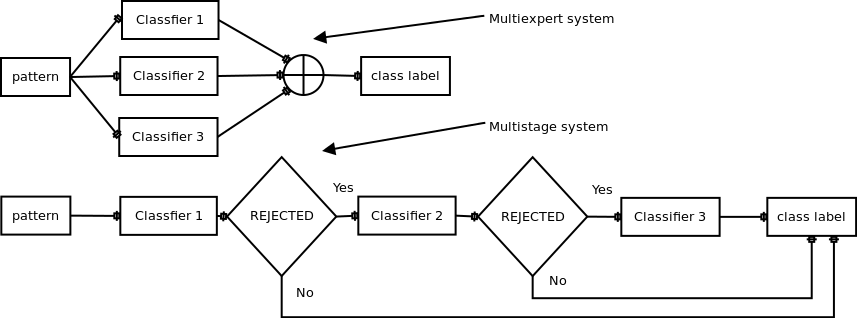
\includegraphics{rys/hybrid}
	\end{center}
	\caption{Hybrid parallel genetic algorithm-schematic illustration}
	\label{fig:hybrid}
\end{figure}
